\title{LEZIONE 19 21/05/20}
\textbf{link} \href{https://web.microsoftstream.com/video/9329ad3d-c8a8-48ab-b415-668ff6193e36?list=user&userId=cfe0965d-9a7c-40e2-be6e-f078296a1914}{clicca qui}
\section{Patter pure HTML vs RIA}
Architettura THIN:
\begin{center}
    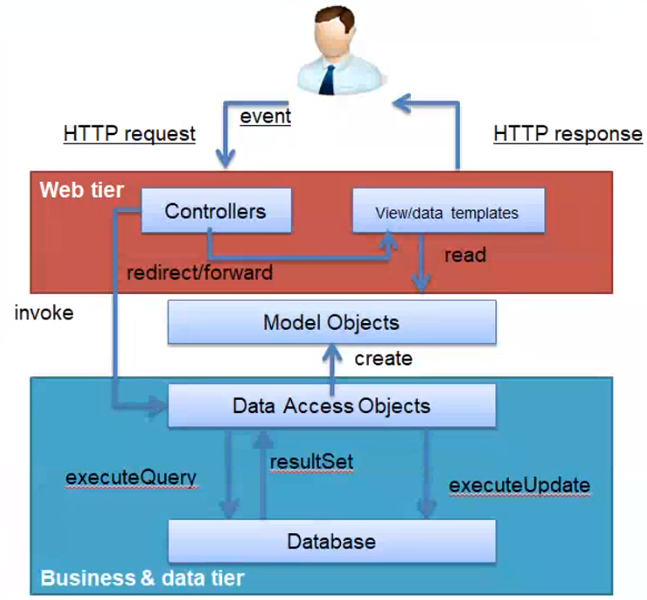
\includegraphics[height=4cm]{../lezione19/img1.PNG}
\end{center}
Architettura FAT:
\begin{center}
    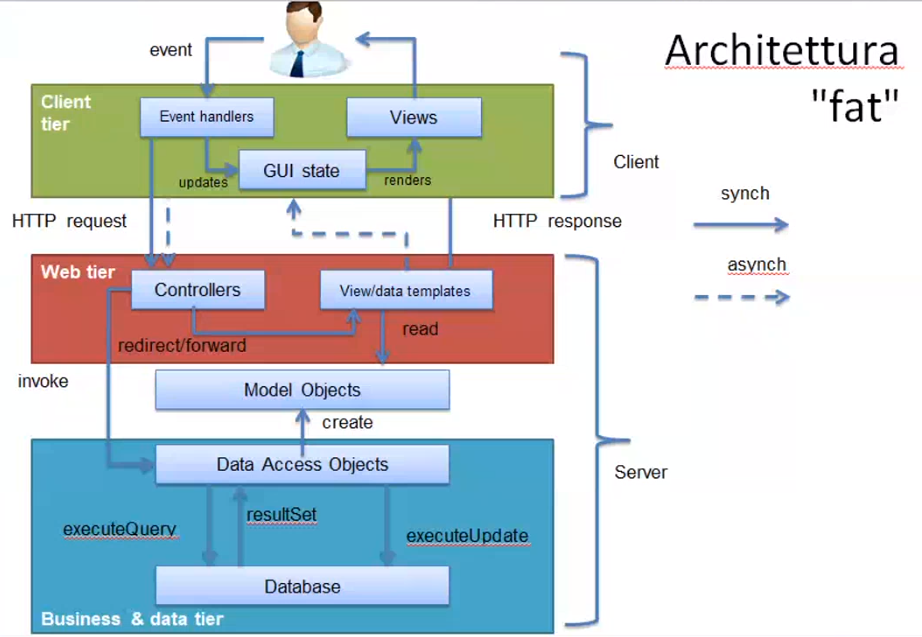
\includegraphics[height=5cm]{../lezione19/img2.PNG}
\end{center} 
Differenze negli eventi.\newline
\begin{multicols}{2}
Pure HTML:
\begin{itemize}
    \item gli eventi sono richieste HTTP;
    \item gli eventi provengono dal client;
    \item gli eventi sono creati dal browser che gestisce per default gli elementi ancora e i buttoni di submit;
    \item gli eventi sono ricevuti dal web server che li inoltra al servlet container (tomcat).
\end{itemize}
\vfill\null
\columnbreak
RIA:
\begin{itemize}
    \item gli eventi sono eventi di DOM e HTML API;
    \item gli eventi provengono dal browser (oggetto window) o dal server (response HTTP);
    \item gli eventi sono prodotti dall'interazione dell'utente o dall'interfaccia di rete (oggetto XMLHttpRequest);
    \item gli eventi sono dal browser e notificati al gestore tramite l'oggetto contenitore window.
\end{itemize}
\end{multicols}
Mappatura degli eventi:
\begin{multicols}{2}
Pure HTML:
\begin{itemize}
    \item il risponditoe è una servlet (controller);
    \item l'associazione tra evento e risponditore è configurata fuori dall'applicazione (web.xml).
\end{itemize}
\vfill\null
\columnbreak
RIA:
\begin{itemize}
    \item il risponditore è una funzione JavaScript;
    \item l'associazione tra evento e risponditore è a carico del programmatore (addEventListener).
\end{itemize}
\end{multicols}
Risposta agli eventi:
\begin{multicols}{2}
Pure HTML:
\begin{itemize}
    \item la risposta agli eventi è sincrona: il client si sospende e attende la response HTTP;
    \item la response HTTP può rimpiazzare il contenuto della pagina corrente oppure forzare l'emissione di una nuova request (redirect);
    \item la response HTTP, il suo stato e il suo contenuto sono gestiti dal browser;
    \item a lato server avvengono sia la trattazione della richiesta sia la selezione della prossima vista.
\end{itemize}
\vfill\null
\columnbreak
RIA:
\begin{itemize}
    \item eventi di interazione: la funzione che risponde può operare solo a lato client oppure creare una richiesta al server, tipicamente asincrona;
    \item eventi di callback: la response HTTP, il suo stato e il suo contenuto sono gestiti dalla funzione che tratta l'evento.
    \item a lato server avviene la trattazione della richiesta;
    \item a lato client avviene la selezione della prossima vista: servlet manda response code e dati, la callback decide la prossima vista.
\end{itemize}
\end{multicols}
Cambio della vista:
\begin{multicols}{2}
Pure HTML:
\begin{itemize}
    \item decisa a lato server;
    \item resonse.getWriter.println, sendError, sendRedirect forzano il cambio integrale del contenuto della vista corrente o la richiesta di una nuova vista;
\end{itemize}
\vfill\null
\columnbreak
RIA:
\begin{itemize}
    \item decisa a lato client;
    \item la proprietà window.location.href permette la sostituzione della vista corrente;
\end{itemize}
\end{multicols}
Submit e risultato:
\begin{multicols}{2}
Pure HTML:
\begin{itemize}
    \item per default la history del browser registra le richieste emesse (URL, POST data\dots);
    \item dopo l'invocazione con metodo POST (passo 1) bisogna fare una nuova richiesta (passo 2) per una nuova pagina che mostri il risultato;
    \item altrimenti il rinfresco della pagina iniziale del processo rimanda la richiesta POST.
\end{itemize}
\vfill\null
\columnbreak
RIA:
\begin{itemize}
    \item la pagina formula una richiesta POST asincrona;
    \item la richiesta asincrona non cambia window.location.href;
    \item l'eventuale rinfresco della pagina produce la visualizzazione della stessa pagina;
    \item il risultato della richiesta POST è visualizzato nella stessa pagina dalla funzione di callbacl deòòa richiesta asincrona;
    \item NB: per ragioni storiche la servlet che gestisca la chiamata asincrona deve essere annotata con @MultipartConfig.
\end{itemize}
\end{multicols}
Presentazione del contenuto dinamico:
\begin{multicols}{2}
Pure HTML:
\begin{itemize}
    \item il controller orchestra l'estrazione del contenuto dinamico, aggiorna il modello e cede il controllo alla view;
    \item la view inserisce il contenuto nel template;
    \item il template attualizzato con il contenuto dinamico viene inviato come response al client;
    \item il browser usa la response per aggiornare l'intera pagina.
\end{itemize}
\vfill\null
\columnbreak
RIA:
\begin{itemize}
    \item il controller orchestra l'estrazione del contenuto dinamico, lo formatta (in JSON) e lo invia come response;
    \item la funzioen di callback del gestore dell'evento attualizza il contenuto della pagina con il contenuto della response.
\end{itemize}
\end{multicols}
Passaggio parametri e stato dell'ultima interazione:
\begin{multicols}{2}
Pure HTML:
\begin{itemize}
    \item quando un evento produce parametri questi sono comunicati al componente che li consuma mediante la request HTTP, anche se servono all'interno della stessa pagina;
    \item è un metodo di preservazione dello stato dell'applicazione di breve termine (dell'ultima interazione), per esempio per preservare la selezione di un elemento da un elenco che aggiorna il contenuto della stessa o di un'altra pagina;
    \item per lo stato di lungo termine (più di un'interazione) serve la sessione o il database. 
\end{itemize}
\vfill\null
\columnbreak
RIA:
\begin{itemize}
    \item quanddo un evento produce parametri che servono all'interno della stessa pagina questi sono preservati come parte dello stato della pagina mediante variabili dei componenti o parametri delle loro funzioni, per esempio la selezione di un elemento da un elenco che aggiorna il contenuto della stessa pagina.
\end{itemize}
\end{multicols}
Mantenimento dello stato:
\begin{multicols}{2}
Pure HTML:
\begin{itemize}
    \item quando deve essere preservata informazione per più di un'interazione si usa la sessione del server;
    \item il controller può creare, vericare e terminare la sessione;
    \item il client può solo trasmettere il proprio session ID.
\end{itemize}
\vfill\null
\columnbreak
RIA:
\begin{itemize}
    \item quando deve essere preservata informazione per più d un'interazione si usa la memoria persistente del client (localStorage e sessionStorage);
    \item il client può creare, verificare e terminare la sessione;
    \item il server può ricevere il contenuto dello stato se necessario, per esempio creare un ordine persistente dai prodotti temporanemente nel carrello.
\end{itemize}
\end{multicols}
\ \newline
N.B. si trovano esempi completi di ognuno di questi concetti nelle slide del prof di questa lezione.